
\documentclass{article}
\usepackage{hyperref}
\usepackage{amsmath}
\usepackage{graphicx}
\usepackage{float}


\begin{document}
\section{Introduction}
In this assignment, I simulate a gas container with $size=30*30$ using velocity-verlet ODE algorithm.
\section{Velocity-Verlet Algorithm}
\begin{equation}
   x_{n+1}=x_n+v_nh-\frac{1}{2}x_nh^2
\end{equation}
\begin{equation}
    v_{n+1}=v_n-\frac{1}{2}(x_n+x_{n+1})h
\end{equation}
\section{Molecular Dynamics}
Assume a gas container that at first all of particles are in the left part of it. After a while, it will spread in the container. 
\begin{figure}[H]
    \centering
    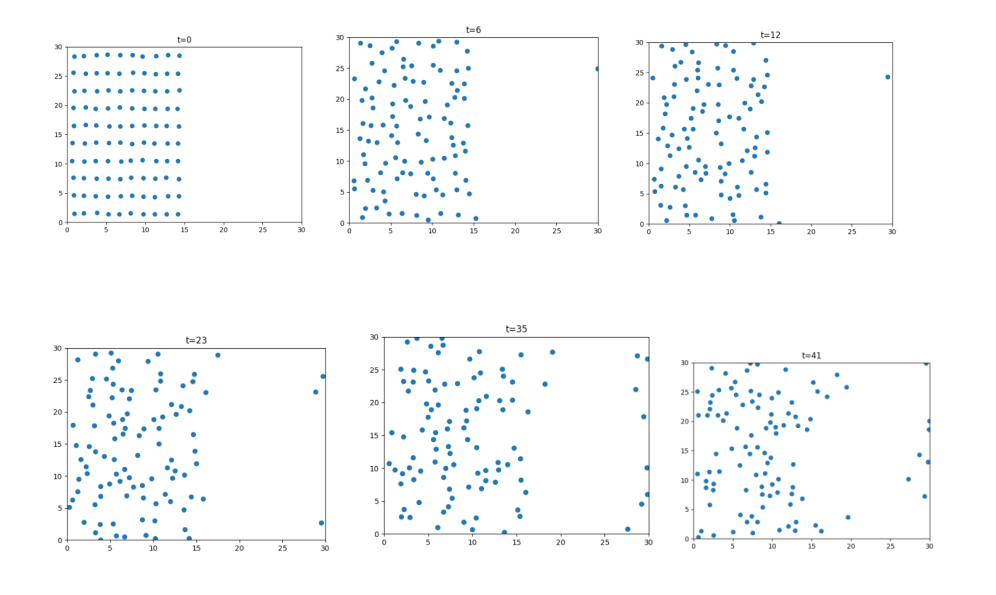
\includegraphics[width=1\linewidth]{gas.PNG}
    \vspace{-1cm}
    \caption{evolution of our gas container, the initial configuration is a simple cubic lattice on the left side of the container.}
\end{figure}
\section{Equilibrium}
\begin{figure}[H]
    \centering
    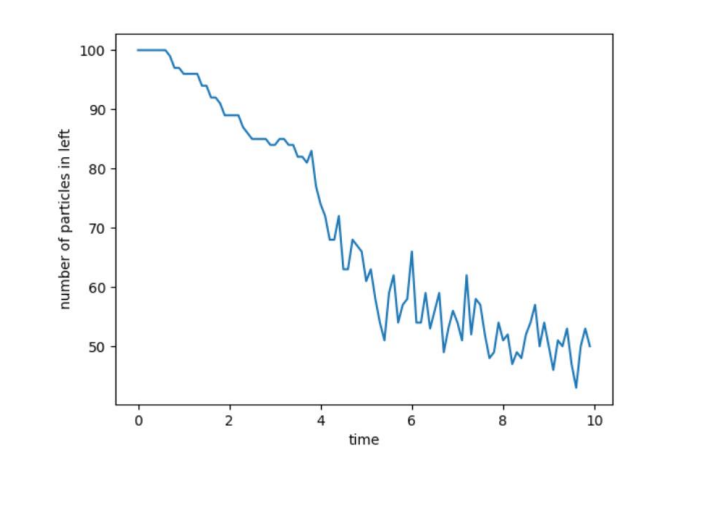
\includegraphics[width=1\linewidth]{gas2.PNG}
    \vspace{-1cm}
    \caption{The ratio of the particles on the left side of the container to the total number of particles starts out equal to 1.0.}
\end{figure}
\section{Conservation of Energy}
In this section, I show the conservation of energy. For calculating the potential energy, Lennard-Jones Potential is used:\\
\begin{equation}
    V_{LJ}=4\epsilon[(\frac{\sigma}{r})^{12}-(\frac{\sigma}{r})^6]
\end{equation}
where r is the distance between each of two particles which reinforced each other.\\
For kinetic energy we have:\\
\begin{equation}
    K = \sum_i \frac{1}{2} v_i^2
\end{equation}
\section{Van der Waals Equation}
\begin{equation}
    (P+a\frac{n^2}{v^2})(V-nb)=nRT
\end{equation}
Where P and V are pressure and volume respectively, and a and b are constants. It could be calculated that\\
\begin{equation}
    P=\frac{1}{V/N-b^*}T-\frac{N^2}{V^2}a^*
\end{equation}
In this section, Van der Waals Equation is simulated and P-T graph is shown. For our gas $a^*=2.26$ and $b^*=1.37$.
\end{document}